% !TEX root = project_proposal.tex
%
%  PACKAGE IMPORTS
%
\documentclass{article} % For LaTeX2e
\usepackage{iclr2022_conference,times}
%%%%% NEW MATH DEFINITIONS %%%%%

\usepackage{amsmath,amsfonts,bm}

% Mark sections of captions for referring to divisions of figures
\newcommand{\figleft}{{\em (Left)}}
\newcommand{\figcenter}{{\em (Center)}}
\newcommand{\figright}{{\em (Right)}}
\newcommand{\figtop}{{\em (Top)}}
\newcommand{\figbottom}{{\em (Bottom)}}
\newcommand{\captiona}{{\em (a)}}
\newcommand{\captionb}{{\em (b)}}
\newcommand{\captionc}{{\em (c)}}
\newcommand{\captiond}{{\em (d)}}

% Highlight a newly defined term
\newcommand{\newterm}[1]{{\bf #1}}


% Figure reference, lower-case.
\def\figref#1{figure~\ref{#1}}
% Figure reference, capital. For start of sentence
\def\Figref#1{Figure~\ref{#1}}
\def\twofigref#1#2{figures \ref{#1} and \ref{#2}}
\def\quadfigref#1#2#3#4{figures \ref{#1}, \ref{#2}, \ref{#3} and \ref{#4}}
% Section reference, lower-case.
\def\secref#1{section~\ref{#1}}
% Section reference, capital.
\def\Secref#1{Section~\ref{#1}}
% Reference to two sections.
\def\twosecrefs#1#2{sections \ref{#1} and \ref{#2}}
% Reference to three sections.
\def\secrefs#1#2#3{sections \ref{#1}, \ref{#2} and \ref{#3}}
% Reference to an equation, lower-case.
\def\eqref#1{equation~\ref{#1}}
% Reference to an equation, upper case
\def\Eqref#1{Equation~\ref{#1}}
% A raw reference to an equation---avoid using if possible
\def\plaineqref#1{\ref{#1}}
% Reference to a chapter, lower-case.
\def\chapref#1{chapter~\ref{#1}}
% Reference to an equation, upper case.
\def\Chapref#1{Chapter~\ref{#1}}
% Reference to a range of chapters
\def\rangechapref#1#2{chapters\ref{#1}--\ref{#2}}
% Reference to an algorithm, lower-case.
\def\algref#1{algorithm~\ref{#1}}
% Reference to an algorithm, upper case.
\def\Algref#1{Algorithm~\ref{#1}}
\def\twoalgref#1#2{algorithms \ref{#1} and \ref{#2}}
\def\Twoalgref#1#2{Algorithms \ref{#1} and \ref{#2}}
% Reference to a part, lower case
\def\partref#1{part~\ref{#1}}
% Reference to a part, upper case
\def\Partref#1{Part~\ref{#1}}
\def\twopartref#1#2{parts \ref{#1} and \ref{#2}}

\def\ceil#1{\lceil #1 \rceil}
\def\floor#1{\lfloor #1 \rfloor}
\def\1{\bm{1}}
\newcommand{\train}{\mathcal{D}}
\newcommand{\valid}{\mathcal{D_{\mathrm{valid}}}}
\newcommand{\test}{\mathcal{D_{\mathrm{test}}}}

\def\eps{{\epsilon}}


% Random variables
\def\reta{{\textnormal{$\eta$}}}
\def\ra{{\textnormal{a}}}
\def\rb{{\textnormal{b}}}
\def\rc{{\textnormal{c}}}
\def\rd{{\textnormal{d}}}
\def\re{{\textnormal{e}}}
\def\rf{{\textnormal{f}}}
\def\rg{{\textnormal{g}}}
\def\rh{{\textnormal{h}}}
\def\ri{{\textnormal{i}}}
\def\rj{{\textnormal{j}}}
\def\rk{{\textnormal{k}}}
\def\rl{{\textnormal{l}}}
% rm is already a command, just don't name any random variables m
\def\rn{{\textnormal{n}}}
\def\ro{{\textnormal{o}}}
\def\rp{{\textnormal{p}}}
\def\rq{{\textnormal{q}}}
\def\rr{{\textnormal{r}}}
\def\rs{{\textnormal{s}}}
\def\rt{{\textnormal{t}}}
\def\ru{{\textnormal{u}}}
\def\rv{{\textnormal{v}}}
\def\rw{{\textnormal{w}}}
\def\rx{{\textnormal{x}}}
\def\ry{{\textnormal{y}}}
\def\rz{{\textnormal{z}}}

% Random vectors
\def\rvepsilon{{\mathbf{\epsilon}}}
\def\rvtheta{{\mathbf{\theta}}}
\def\rva{{\mathbf{a}}}
\def\rvb{{\mathbf{b}}}
\def\rvc{{\mathbf{c}}}
\def\rvd{{\mathbf{d}}}
\def\rve{{\mathbf{e}}}
\def\rvf{{\mathbf{f}}}
\def\rvg{{\mathbf{g}}}
\def\rvh{{\mathbf{h}}}
\def\rvu{{\mathbf{i}}}
\def\rvj{{\mathbf{j}}}
\def\rvk{{\mathbf{k}}}
\def\rvl{{\mathbf{l}}}
\def\rvm{{\mathbf{m}}}
\def\rvn{{\mathbf{n}}}
\def\rvo{{\mathbf{o}}}
\def\rvp{{\mathbf{p}}}
\def\rvq{{\mathbf{q}}}
\def\rvr{{\mathbf{r}}}
\def\rvs{{\mathbf{s}}}
\def\rvt{{\mathbf{t}}}
\def\rvu{{\mathbf{u}}}
\def\rvv{{\mathbf{v}}}
\def\rvw{{\mathbf{w}}}
\def\rvx{{\mathbf{x}}}
\def\rvy{{\mathbf{y}}}
\def\rvz{{\mathbf{z}}}

% Elements of random vectors
\def\erva{{\textnormal{a}}}
\def\ervb{{\textnormal{b}}}
\def\ervc{{\textnormal{c}}}
\def\ervd{{\textnormal{d}}}
\def\erve{{\textnormal{e}}}
\def\ervf{{\textnormal{f}}}
\def\ervg{{\textnormal{g}}}
\def\ervh{{\textnormal{h}}}
\def\ervi{{\textnormal{i}}}
\def\ervj{{\textnormal{j}}}
\def\ervk{{\textnormal{k}}}
\def\ervl{{\textnormal{l}}}
\def\ervm{{\textnormal{m}}}
\def\ervn{{\textnormal{n}}}
\def\ervo{{\textnormal{o}}}
\def\ervp{{\textnormal{p}}}
\def\ervq{{\textnormal{q}}}
\def\ervr{{\textnormal{r}}}
\def\ervs{{\textnormal{s}}}
\def\ervt{{\textnormal{t}}}
\def\ervu{{\textnormal{u}}}
\def\ervv{{\textnormal{v}}}
\def\ervw{{\textnormal{w}}}
\def\ervx{{\textnormal{x}}}
\def\ervy{{\textnormal{y}}}
\def\ervz{{\textnormal{z}}}

% Random matrices
\def\rmA{{\mathbf{A}}}
\def\rmB{{\mathbf{B}}}
\def\rmC{{\mathbf{C}}}
\def\rmD{{\mathbf{D}}}
\def\rmE{{\mathbf{E}}}
\def\rmF{{\mathbf{F}}}
\def\rmG{{\mathbf{G}}}
\def\rmH{{\mathbf{H}}}
\def\rmI{{\mathbf{I}}}
\def\rmJ{{\mathbf{J}}}
\def\rmK{{\mathbf{K}}}
\def\rmL{{\mathbf{L}}}
\def\rmM{{\mathbf{M}}}
\def\rmN{{\mathbf{N}}}
\def\rmO{{\mathbf{O}}}
\def\rmP{{\mathbf{P}}}
\def\rmQ{{\mathbf{Q}}}
\def\rmR{{\mathbf{R}}}
\def\rmS{{\mathbf{S}}}
\def\rmT{{\mathbf{T}}}
\def\rmU{{\mathbf{U}}}
\def\rmV{{\mathbf{V}}}
\def\rmW{{\mathbf{W}}}
\def\rmX{{\mathbf{X}}}
\def\rmY{{\mathbf{Y}}}
\def\rmZ{{\mathbf{Z}}}

% Elements of random matrices
\def\ermA{{\textnormal{A}}}
\def\ermB{{\textnormal{B}}}
\def\ermC{{\textnormal{C}}}
\def\ermD{{\textnormal{D}}}
\def\ermE{{\textnormal{E}}}
\def\ermF{{\textnormal{F}}}
\def\ermG{{\textnormal{G}}}
\def\ermH{{\textnormal{H}}}
\def\ermI{{\textnormal{I}}}
\def\ermJ{{\textnormal{J}}}
\def\ermK{{\textnormal{K}}}
\def\ermL{{\textnormal{L}}}
\def\ermM{{\textnormal{M}}}
\def\ermN{{\textnormal{N}}}
\def\ermO{{\textnormal{O}}}
\def\ermP{{\textnormal{P}}}
\def\ermQ{{\textnormal{Q}}}
\def\ermR{{\textnormal{R}}}
\def\ermS{{\textnormal{S}}}
\def\ermT{{\textnormal{T}}}
\def\ermU{{\textnormal{U}}}
\def\ermV{{\textnormal{V}}}
\def\ermW{{\textnormal{W}}}
\def\ermX{{\textnormal{X}}}
\def\ermY{{\textnormal{Y}}}
\def\ermZ{{\textnormal{Z}}}

% Vectors
\def\vzero{{\bm{0}}}
\def\vone{{\bm{1}}}
\def\vmu{{\bm{\mu}}}
\def\vtheta{{\bm{\theta}}}
\def\va{{\bm{a}}}
\def\vb{{\bm{b}}}
\def\vc{{\bm{c}}}
\def\vd{{\bm{d}}}
\def\ve{{\bm{e}}}
\def\vf{{\bm{f}}}
\def\vg{{\bm{g}}}
\def\vh{{\bm{h}}}
\def\vi{{\bm{i}}}
\def\vj{{\bm{j}}}
\def\vk{{\bm{k}}}
\def\vl{{\bm{l}}}
\def\vm{{\bm{m}}}
\def\vn{{\bm{n}}}
\def\vo{{\bm{o}}}
\def\vp{{\bm{p}}}
\def\vq{{\bm{q}}}
\def\vr{{\bm{r}}}
\def\vs{{\bm{s}}}
\def\vt{{\bm{t}}}
\def\vu{{\bm{u}}}
\def\vv{{\bm{v}}}
\def\vw{{\bm{w}}}
\def\vx{{\bm{x}}}
\def\vy{{\bm{y}}}
\def\vz{{\bm{z}}}

% Elements of vectors
\def\evalpha{{\alpha}}
\def\evbeta{{\beta}}
\def\evepsilon{{\epsilon}}
\def\evlambda{{\lambda}}
\def\evomega{{\omega}}
\def\evmu{{\mu}}
\def\evpsi{{\psi}}
\def\evsigma{{\sigma}}
\def\evtheta{{\theta}}
\def\eva{{a}}
\def\evb{{b}}
\def\evc{{c}}
\def\evd{{d}}
\def\eve{{e}}
\def\evf{{f}}
\def\evg{{g}}
\def\evh{{h}}
\def\evi{{i}}
\def\evj{{j}}
\def\evk{{k}}
\def\evl{{l}}
\def\evm{{m}}
\def\evn{{n}}
\def\evo{{o}}
\def\evp{{p}}
\def\evq{{q}}
\def\evr{{r}}
\def\evs{{s}}
\def\evt{{t}}
\def\evu{{u}}
\def\evv{{v}}
\def\evw{{w}}
\def\evx{{x}}
\def\evy{{y}}
\def\evz{{z}}

% Matrix
\def\mA{{\bm{A}}}
\def\mB{{\bm{B}}}
\def\mC{{\bm{C}}}
\def\mD{{\bm{D}}}
\def\mE{{\bm{E}}}
\def\mF{{\bm{F}}}
\def\mG{{\bm{G}}}
\def\mH{{\bm{H}}}
\def\mI{{\bm{I}}}
\def\mJ{{\bm{J}}}
\def\mK{{\bm{K}}}
\def\mL{{\bm{L}}}
\def\mM{{\bm{M}}}
\def\mN{{\bm{N}}}
\def\mO{{\bm{O}}}
\def\mP{{\bm{P}}}
\def\mQ{{\bm{Q}}}
\def\mR{{\bm{R}}}
\def\mS{{\bm{S}}}
\def\mT{{\bm{T}}}
\def\mU{{\bm{U}}}
\def\mV{{\bm{V}}}
\def\mW{{\bm{W}}}
\def\mX{{\bm{X}}}
\def\mY{{\bm{Y}}}
\def\mZ{{\bm{Z}}}
\def\mBeta{{\bm{\beta}}}
\def\mPhi{{\bm{\Phi}}}
\def\mLambda{{\bm{\Lambda}}}
\def\mSigma{{\bm{\Sigma}}}

% Tensor
\DeclareMathAlphabet{\mathsfit}{\encodingdefault}{\sfdefault}{m}{sl}
\SetMathAlphabet{\mathsfit}{bold}{\encodingdefault}{\sfdefault}{bx}{n}
\newcommand{\tens}[1]{\bm{\mathsfit{#1}}}
\def\tA{{\tens{A}}}
\def\tB{{\tens{B}}}
\def\tC{{\tens{C}}}
\def\tD{{\tens{D}}}
\def\tE{{\tens{E}}}
\def\tF{{\tens{F}}}
\def\tG{{\tens{G}}}
\def\tH{{\tens{H}}}
\def\tI{{\tens{I}}}
\def\tJ{{\tens{J}}}
\def\tK{{\tens{K}}}
\def\tL{{\tens{L}}}
\def\tM{{\tens{M}}}
\def\tN{{\tens{N}}}
\def\tO{{\tens{O}}}
\def\tP{{\tens{P}}}
\def\tQ{{\tens{Q}}}
\def\tR{{\tens{R}}}
\def\tS{{\tens{S}}}
\def\tT{{\tens{T}}}
\def\tU{{\tens{U}}}
\def\tV{{\tens{V}}}
\def\tW{{\tens{W}}}
\def\tX{{\tens{X}}}
\def\tY{{\tens{Y}}}
\def\tZ{{\tens{Z}}}


% Graph
\def\gA{{\mathcal{A}}}
\def\gB{{\mathcal{B}}}
\def\gC{{\mathcal{C}}}
\def\gD{{\mathcal{D}}}
\def\gE{{\mathcal{E}}}
\def\gF{{\mathcal{F}}}
\def\gG{{\mathcal{G}}}
\def\gH{{\mathcal{H}}}
\def\gI{{\mathcal{I}}}
\def\gJ{{\mathcal{J}}}
\def\gK{{\mathcal{K}}}
\def\gL{{\mathcal{L}}}
\def\gM{{\mathcal{M}}}
\def\gN{{\mathcal{N}}}
\def\gO{{\mathcal{O}}}
\def\gP{{\mathcal{P}}}
\def\gQ{{\mathcal{Q}}}
\def\gR{{\mathcal{R}}}
\def\gS{{\mathcal{S}}}
\def\gT{{\mathcal{T}}}
\def\gU{{\mathcal{U}}}
\def\gV{{\mathcal{V}}}
\def\gW{{\mathcal{W}}}
\def\gX{{\mathcal{X}}}
\def\gY{{\mathcal{Y}}}
\def\gZ{{\mathcal{Z}}}

% Sets
\def\sA{{\mathbb{A}}}
\def\sB{{\mathbb{B}}}
\def\sC{{\mathbb{C}}}
\def\sD{{\mathbb{D}}}
% Don't use a set called E, because this would be the same as our symbol
% for expectation.
\def\sF{{\mathbb{F}}}
\def\sG{{\mathbb{G}}}
\def\sH{{\mathbb{H}}}
\def\sI{{\mathbb{I}}}
\def\sJ{{\mathbb{J}}}
\def\sK{{\mathbb{K}}}
\def\sL{{\mathbb{L}}}
\def\sM{{\mathbb{M}}}
\def\sN{{\mathbb{N}}}
\def\sO{{\mathbb{O}}}
\def\sP{{\mathbb{P}}}
\def\sQ{{\mathbb{Q}}}
\def\sR{{\mathbb{R}}}
\def\sS{{\mathbb{S}}}
\def\sT{{\mathbb{T}}}
\def\sU{{\mathbb{U}}}
\def\sV{{\mathbb{V}}}
\def\sW{{\mathbb{W}}}
\def\sX{{\mathbb{X}}}
\def\sY{{\mathbb{Y}}}
\def\sZ{{\mathbb{Z}}}

% Entries of a matrix
\def\emLambda{{\Lambda}}
\def\emA{{A}}
\def\emB{{B}}
\def\emC{{C}}
\def\emD{{D}}
\def\emE{{E}}
\def\emF{{F}}
\def\emG{{G}}
\def\emH{{H}}
\def\emI{{I}}
\def\emJ{{J}}
\def\emK{{K}}
\def\emL{{L}}
\def\emM{{M}}
\def\emN{{N}}
\def\emO{{O}}
\def\emP{{P}}
\def\emQ{{Q}}
\def\emR{{R}}
\def\emS{{S}}
\def\emT{{T}}
\def\emU{{U}}
\def\emV{{V}}
\def\emW{{W}}
\def\emX{{X}}
\def\emY{{Y}}
\def\emZ{{Z}}
\def\emSigma{{\Sigma}}

% entries of a tensor
% Same font as tensor, without \bm wrapper
\newcommand{\etens}[1]{\mathsfit{#1}}
\def\etLambda{{\etens{\Lambda}}}
\def\etA{{\etens{A}}}
\def\etB{{\etens{B}}}
\def\etC{{\etens{C}}}
\def\etD{{\etens{D}}}
\def\etE{{\etens{E}}}
\def\etF{{\etens{F}}}
\def\etG{{\etens{G}}}
\def\etH{{\etens{H}}}
\def\etI{{\etens{I}}}
\def\etJ{{\etens{J}}}
\def\etK{{\etens{K}}}
\def\etL{{\etens{L}}}
\def\etM{{\etens{M}}}
\def\etN{{\etens{N}}}
\def\etO{{\etens{O}}}
\def\etP{{\etens{P}}}
\def\etQ{{\etens{Q}}}
\def\etR{{\etens{R}}}
\def\etS{{\etens{S}}}
\def\etT{{\etens{T}}}
\def\etU{{\etens{U}}}
\def\etV{{\etens{V}}}
\def\etW{{\etens{W}}}
\def\etX{{\etens{X}}}
\def\etY{{\etens{Y}}}
\def\etZ{{\etens{Z}}}

% The true underlying data generating distribution
\newcommand{\pdata}{p_{\rm{data}}}
% The empirical distribution defined by the training set
\newcommand{\ptrain}{\hat{p}_{\rm{data}}}
\newcommand{\Ptrain}{\hat{P}_{\rm{data}}}
% The model distribution
\newcommand{\pmodel}{p_{\rm{model}}}
\newcommand{\Pmodel}{P_{\rm{model}}}
\newcommand{\ptildemodel}{\tilde{p}_{\rm{model}}}
% Stochastic autoencoder distributions
\newcommand{\pencode}{p_{\rm{encoder}}}
\newcommand{\pdecode}{p_{\rm{decoder}}}
\newcommand{\precons}{p_{\rm{reconstruct}}}

\newcommand{\laplace}{\mathrm{Laplace}} % Laplace distribution

\newcommand{\E}{\mathbb{E}}
\newcommand{\Ls}{\mathcal{L}}
\newcommand{\R}{\mathbb{R}}
\newcommand{\emp}{\tilde{p}}
\newcommand{\lr}{\alpha}
\newcommand{\reg}{\lambda}
\newcommand{\rect}{\mathrm{rectifier}}
\newcommand{\softmax}{\mathrm{softmax}}
\newcommand{\sigmoid}{\sigma}
\newcommand{\softplus}{\zeta}
\newcommand{\KL}{D_{\mathrm{KL}}}
\newcommand{\Var}{\mathrm{Var}}
\newcommand{\standarderror}{\mathrm{SE}}
\newcommand{\Cov}{\mathrm{Cov}}
% Wolfram Mathworld says $L^2$ is for function spaces and $\ell^2$ is for vectors
% But then they seem to use $L^2$ for vectors throughout the site, and so does
% wikipedia.
\newcommand{\normlzero}{L^0}
\newcommand{\normlone}{L^1}
\newcommand{\normltwo}{L^2}
\newcommand{\normlp}{L^p}
\newcommand{\normmax}{L^\infty}

\newcommand{\parents}{Pa} % See usage in notation.tex. Chosen to match Daphne's book.

\DeclareMathOperator*{\argmax}{arg\,max}
\DeclareMathOperator*{\argmin}{arg\,min}

\DeclareMathOperator{\sign}{sign}
\DeclareMathOperator{\Tr}{Tr}
\let\ab\allowbreak


\newcommand{\apsname}{Progress Report}
\newcommand{\gpnumber}{26}

\usepackage{hyperref}
\usepackage{url}
\usepackage{graphicx}
\usepackage[table]{xcolor}

\usepackage{graphicx} % Required for \resizebox
\usepackage{placeins} % Required for \FloatBarrier

%
%  TITLE AND AUTHORS
%
\title{Deep learning approach to  \\ 
mushroom species classification}

\author{Yanni Alan Alevras  \\
Student\# 1009330706 \\
\texttt{yanni.alevras@mail.utoronto.ca} \\
\And
Nicholas Biancolin  \\
Student\# 1009197726 \\
\texttt{n.biancolin@mail.utoronto.ca} \\
\AND
Eric Liu  \\
Student\# 1009098450 \\
\texttt{ey.liu@mail.utoronto.ca} \\
\And
Jason Ruixuan Zhang \\
Student\# 1008997631 \\
\texttt{jasonrx.zhang@mail.utoronto.ca} \\
\AND
}

\newcommand{\fix}{\marginpar{FIX}}
\newcommand{\new}{\marginpar{NEW}}

\iclrfinalcopy

%
%   DOCUMENT STARTS HERE
%

\begin{document}
\maketitle

\section{Project Description}
\label{sec:project_description}

Fungi identification is an increasingly critical task, with implications in food security, industrial use, conservation efforts, and biosafety. However, visual and image classification of fungi is a difficult task due to the wide variety of species. The goal of this project is to develop a deep learning model that can accurately identify macrofungi (fungi with large bodies) based on their genus. 

87 percent of the land in Ontario is Crown Land, filled with expansive forests and a diverse array of plant species. Among these, mushrooms stand out as both common and challenging to identify due to their wide variety and the subtle differences between species.This identification task is particularly crucial because while some mushrooms are edible, others are highly poisonous, potentially posing a significant risk to foragers and nature enthusiasts.

We believe deep learning is a suitable approach for this task as deep learning models have proven to be effective in image classification tasks. Furthermore, there is a robust amount of data available for training, helping to ensure a solid model.


\section{Indvidual Contributions and Responsibilities}
\label{sec:individual_contributions_and_responsibilities}

- How team is working together


-project management software used to communicate/track results


-detailed list of what everyone has worked on, and what they will be working on

Jason:

Set up python environment for the group to work with. Genus grouping to reduce size of dataset. Random forest baseline model with accuracy, precision, recall, F1, and support reports. Baseline Model section of the report..

Yanni:

Researching which forms of data augmentation are most relevant to the project. Data augmentation additions to the dataset. Data Processing and Individual Contributions and Responsibilities sections of the report. 

Eric:

Rough Draft for Primary Model section of the report. handdrawn diagram of structure. Data Separation and Apply Transfer Learning: alexNet. Class Structure, Training Function, Accuracy function. Validation Loss and Graphs.

\begin{center}
\begin{tabular}{ |c|c|c|c| }
\hline
\rowcolor{gray!50}
\textbf{Yanni} & \textbf{Nick} & \textbf{Eric} & \textbf{Jason} \\
\hline


\end{tabular}
\end{center}

\begin{table}[ht]
    \centering
    \resizebox{\textwidth}{!}{%
    \begin{tabular}{|l|c|c|c|c|}
        \hline
        \rowcolor{gray!50}
        \textbf{Project Progress Report} & \textbf{Eric Liu} & \textbf{Jason Zhang} & \textbf{Nicholas Biancolin} & \textbf{Yanni Alevras} \\
        \hline
        \rowcolor{green!50}
        Brief Project Description (June 30th, 11:59 pm) & & & W & \\
        \hline
        \rowcolor{green!50}
        Individual Contributions and Responsibilities (June 30th, 11:59 pm) & & & W & W \\
        \hline
        \rowcolor{green!50}
        Contributions - Data Processing (June 30th, 11:59 pm) & & & & W \\
        \hline
        \rowcolor{green!50}
        Contributions - Baseline Model (June 30th, 11:59 pm) & & W & & \\
        \hline
        \rowcolor{green!50}
        Contributions - Primary Model (June 30th, 11:59 pm) & W & & & \\
        \hline
        \rowcolor{green!50}
        Illustrations (July 1st, 11:59 pm) & W & & & W \\
        \hline
        \rowcolor{green!50}
        Latex format (July 2nd, 11:59 pm) & W & W & W & W \\
        \hline
        \rowcolor{green!50}
        Editing (July 3rd, 11:59 pm) & ED & ED & ED & ED\\
        \hline
        \rowcolor{green!50}
        Final Proofread (July 4th, 6:00 pm) & W & W & W & W \\
        \hline
    \end{tabular}}
    \caption{Project Progress Report Task Breakdown}
\end{table}

\FloatBarrier

\begin{table}[ht]
    \centering
    \resizebox{\textwidth}{!}{%
    \begin{tabular}{|l|c|c|c|c|}
        \hline
        \rowcolor{gray!50}
        \textbf{Project - Training and Testing} & \textbf{Eric Liu} & \textbf{Jason Zhang} & \textbf{Nicholas Biancolin} & \textbf{Yanni Alevras} \\
        \hline
        \rowcolor{red!50}
        In charge of code connection/solving merge conflicts (August 10th, 11:59pm) & W & W & ED & \\
        \hline
        \rowcolor{red!50}
        Data Cleaning (June 16th, 11:59pm) & W & W & & ED \\
        \hline
        \rowcolor{red!50}
        Image Grouping (June 16th, 11:59pm) & ED & & W & ED \\
        \hline
        \rowcolor{red!50}
        Transfer data to training format (June 16th, 11:59pm) & ED & ED & W & \\
        \hline
        \rowcolor{red!50}
        Data annotations, splitting (June 16th, 11:59pm) & W & & & ED \\
        \hline
        \rowcolor{red!50}
        Model implementation (June 19th, 11:59pm) & & W & & ED \\
        \hline
        \rowcolor{red!50}
        CNN architecture (June 19th, 11:59pm) & & ED & & W \\
        \hline
        \rowcolor{red!50}
        Training Loop (June 19th, 11:59pm) & W & W & ED & ED \\
        \hline
        \rowcolor{red!50}
        Hyperparameter adjustments (July 15th, 11:59pm) & W & ED & & W \\
        \hline
        \rowcolor{red!50}
        Training (July 15th, 11:59pm) & W ED & W ED & W & W \\
        \hline
        \rowcolor{red!50}
        Validation (July 15th, 11:59pm) & & W & & ED \\
        \hline
        \rowcolor{red!50}
        Testing (August 10th, 11:59pm) & W & ED & W & \\
        \hline
        \rowcolor{red!50}
        Iterative (if needed) (August 10th, 11:59pm) & & ED & & W \\
        \hline
        \rowcolor{red!50}
        Evaluation (August 10th, 11:59pm) & W & W & W ED & W\\
        \hline
        \rowcolor{red!50}
        Documentation (August 10th, 11:59pm) & W & W & ED & \\
        \hline
        \rowcolor{red!50}
        Resource management (August 3rd, 11:59pm) & & & W & ED \\
        \hline
        \rowcolor{red!50}
        Analyze Result for Presentation and Project (August 3rd, 11:59pm) & W & W & W & W \\
        \hline
    \end{tabular}}
    \caption{Project Training and Testing Task Breakdown}
\end{table}

\FloatBarrier

\begin{table}[ht]
    \centering
    \resizebox{\textwidth}{!}{%
    \begin{tabular}{|l|c|c|c|c|}
        \hline
        \rowcolor{gray!50}
        \textbf{Presentation} & \textbf{Eric Liu} & \textbf{Jason Zhang} & \textbf{Nicholas Biancolin} & \textbf{Yanni Alevras} \\
        \hline
        \rowcolor{red!50}
        Presentation Brainstorm (August 5th, 11:59pm) & W & W & W & W \\
        \hline
        \rowcolor{red!50}
        Problem - slides (August 5th, 11:59pm) & & ED & W & \\
        \hline
        \rowcolor{red!50}
        Data Processing - slides (August 5th, 11:59pm) & W & & & ED \\
        \hline
        \rowcolor{red!50}
        Model - slides (August 5th, 11:59pm) & & W & ED & \\
        \hline
        \rowcolor{red!50}
        Result - slides (August 5th, 11:59pm) & ED & & & W \\
        \hline
        \rowcolor{red!50}
        Slides Editing (August 5th, 11:59pm) & ED & ED & & \\
        \hline
        \rowcolor{red!50}
        Individual Practice (August 7th, 11:59pm) & W & W & W & W\\
        \hline
        \rowcolor{red!50}
        Group Practice (August 7th, 11:59pm) & W & W & W & W \\
        \hline
        \rowcolor{red!50}
        Record Presentation (August 7th, 11:59pm) & W & W & W & W \\
        \hline
        \rowcolor{red!50}
        Editing (August 10th, 11:59pm) & & & W & ED \\
        \hline
    \end{tabular}}
    \caption{Presentation Task Breakdown}
\end{table}

\FloatBarrier

\begin{table}[ht]
    \centering
    \resizebox{\textwidth}{!}{%
    \begin{tabular}{|l|c|c|c|c|}
        \hline
        \rowcolor{gray!50}
        \textbf{Project Final Report} & \textbf{Eric Liu} & \textbf{Jason Zhang} & \textbf{Nicholas Biancolin} & \textbf{Yanni Alevras} \\
        \hline
        \rowcolor{red!50}
        Latex Formatting (August 12th, 11:59pm) & W & W & ED & \\
        \hline
        \rowcolor{red!50}
        Introduction (August 7th, 11:59pm) & & ED & W & W\\
        \hline
        \rowcolor{red!50}
        Illustration (August 7th, 11:59pm) & W & ED & & \\
        \hline
        \rowcolor{red!50}
        Background and Related Work (August 7th, 11:59pm) & & W & ED & ED \\
        \hline
        \rowcolor{red!50}
        Data Processing (August 7th, 11:59pm) & & W & & ED \\
        \hline
        \rowcolor{red!50}
        Architecture (August 7th, 11:59pm) & ED & & W & \\
        \hline
        \rowcolor{red!50}
        Baseline Model (August 7th, 11:59pm) & ED & ED & & W \\
        \hline
        \rowcolor{red!50}
        Qualitative Results (August 7th, 11:59pm) & W & ED & & \\
        \hline
        \rowcolor{red!50}
        Quantitative Results (August 7th, 11:59pm) & & W & & ED \\
        \hline
        \rowcolor{red!50}
        Evaluation of Model (August 7th, 11:59pm) & W & & W ED& ED\\
        \hline
        \rowcolor{red!50}
        Discussion (August 7th, 11:59pm) & ED & W & & W\\
        \hline
        \rowcolor{red!50}
        Ethical Considerations (August 7th, 11:59pm) & & W& & ED \\
        \hline
        \rowcolor{red!50}
        Project Difficulty (August 7th, 11:59pm) & W & ED & & \\
        \hline
        \rowcolor{red!50}
        Editing (August 12th, 11:59pm) & ED & & ED & W \\
        \hline
        \rowcolor{red!50}
        Final Proofread (August 14th, 11:59pm) & W & W & W & W\\
        \hline
    \end{tabular}}
    \caption{Project Final Report Task Breakdown}
\end{table}

\FloatBarrier

\section{Notable Contribution}
\label{sec:notable_contribution}

\subsection{Data Processing}

<<<<<<< HEAD
The dataset contains 509 species. Stated in our project proposal, due to some low amount of sample imaging for some species we decided to group by genus, and keep the top 15 genera with the largest datasets. This genus grouping was done through iterating all of the species in the dataset, and moving all of the data into a new directory for that genus. These directories were then ordered by size, and the top 15 were kept.


To artificially increase the amount of data in our dataset, we used data augmentation, creating a copy of each sample with a horizontal flip, 90 degree rotation, 180 degree rotation, 270 degree rotation, gaussian noise, and random erasing (small black rectangles). These methods were preferred over others such as kernel filters, lowering the quality of an image. Since these mushrooms can be identified based on specific visual traits found within their genus, high detail in the training images are necessary to allow for differentiation between the different genera. Due to this, prioritizing the quality of the image was necessary. In addition, our model is colour agnostic, so having a method like color space transformations are not necessary, and would allow for too many almost duplicate images in the dataset. Some simple methods were the flip and rotations, which kept the same image, but just made the model look at it a different way. Gaussian noise was added as a technique to allow the model to draw attention towards the most robust features of the image, relevant to the nature of this dataset where many genera are similar in shape and very based on texture or pattern. Random erasing is important for training with data that varies in resolution. This dataset has mostly high quality images, but some are lower resolution. This method was added for a similar reason as gaussian noise, but instead to train the model to identify more distinct features of one genus to another (Shorten et al., 2019).

\FloatBarrier

\begin{figure}[h]
    \begin{center}
    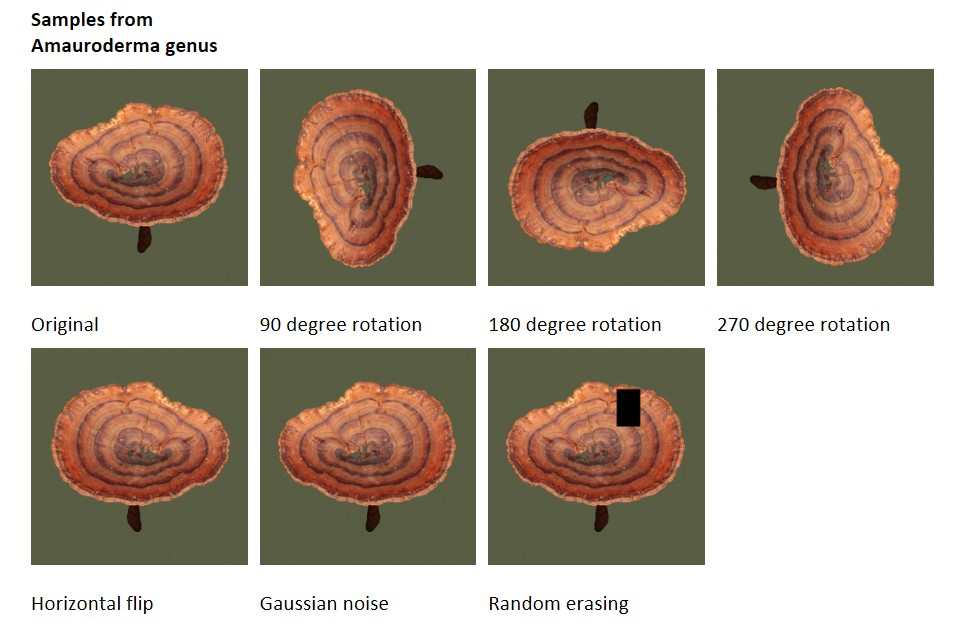
\includegraphics[width=0.9\textwidth]{figures/data_aug.jpg}
    \end{center}
    \caption{Data Augmentation Examples}
\end{figure}

\FloatBarrier

To test this data, it is split into #\% training, #\% validation and #\% testing. Our evaluation metrics consist of accuracy, precision, recall, F1 and support. This is to provide a wider view on the performance of the model, including underrepresented classes.

The biggest challenge for the data processing, was figuring out how much original data we would need, and how much we want to use data processing to increase the amount of data. Including what types of data augmentation we would see fit, explained above. Overall the top 15 genera have around 200-1000 images each, with data augmentation multiplying that my seven.




Primary Model


\subsection{Baseline Model}
Our baseline model is a random forests classifier trained with scikit-learn. As mentioned in our proposal, decision trees like random forest are generally well-suited for multiclass problems \citep{GallRazaviEtAl.IntroductionRandomForests.2012}.

We follow similar processing steps as the primary model, in the following order: a test-train split of 80\%/20\%, feature extraction with HOG, training, and performance assessments. The model uses the same dataset as the primary model with the exclusion of augmented data and additional restrictions on image size (300 x 300) and number of colour channels. The restriction on image size is primarily to reduce training complexity and time.

A conversion to grayscale is necessary to facilitate feature extraction with histogram of oriented gradients (HOG) \citep{AbouelnagaThambirajaEtAl.ObjectDetectionHistogram.2018}, computed with scikit-image. As models like random forest do not automatically perform feature extraction (in comparison to deep convolutional networks, which our primary model uses), this step is done to provide the model with a set of features to learn from. We compute HOG features on both the training and testing set, in line with the process outlined by \cite{Shafi.RandomForestClassification.2023}. We use default hyperparameters for training, with the exception of the number of estimators, which is set to 500, which \cite{Xi.ImageClassificationRecognition.2022} suggests is an optimal amount of trees for increasing accuracy.

Training takes approximately 4 minutes on a CPU. This is significantly faster than the primary model, which takes % get this number

The model has a training accuracy of about 54\%, roughly 10\% worse than the primary model. This is expected, as random forests are generally less accurate than deep learning models for image classification tasks. We also used minimal hyperparameter tuning, which could have otherwise improved the model's performance. A more complicated architecture, like an ensemble model with convolutional feature extraction could have also improved model performance \citep{Xi.ImageClassificationRecognition.2022}.

\begin{figure}[h]
    \begin{center}
    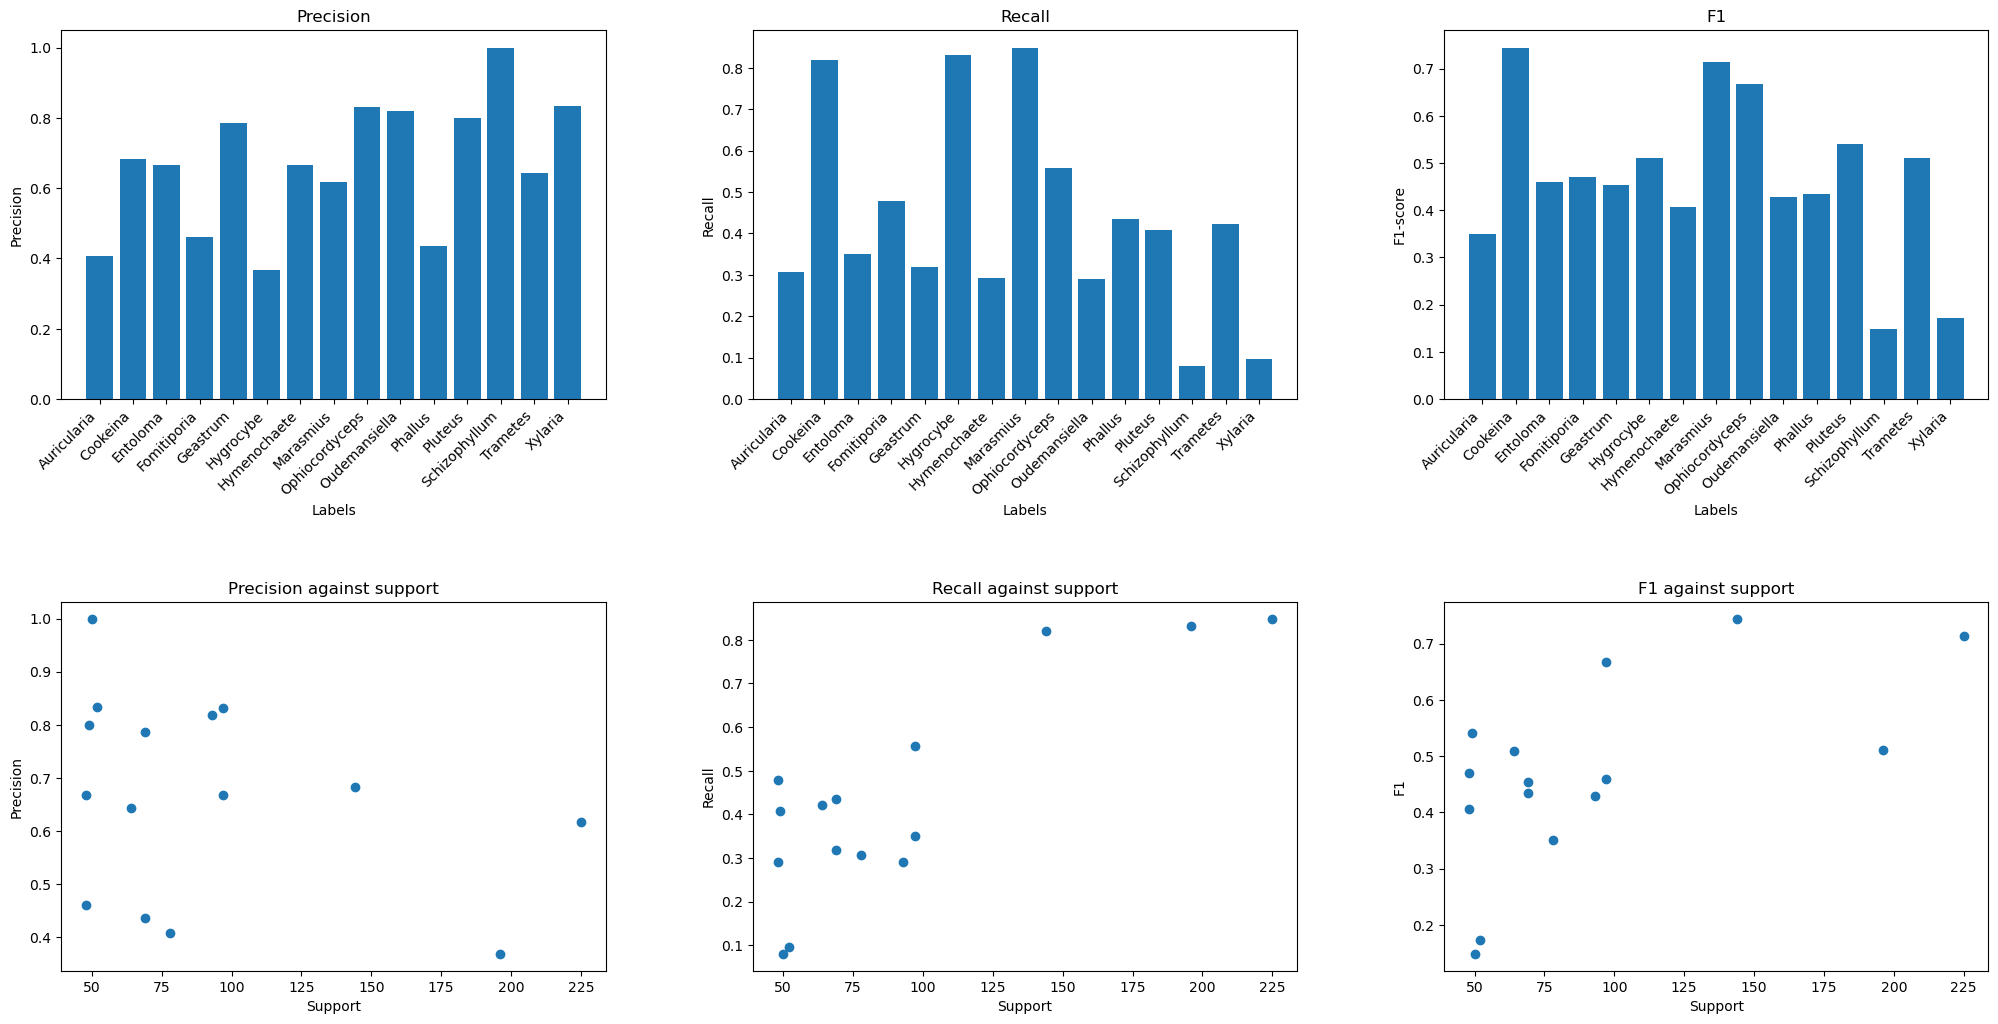
\includegraphics[width=1.0\textwidth]{figures/baseline.png}
    \end{center}
    \caption{Precision, recall, and F1-score for the baseline model}
\end{figure}

The precision, recall, and F1-score are plotted in the following figure. We have an average precision of 0.67, recall of 0.44, and F-score of 0.47. Notably, the recall and F-score data take a similar shape, which lower-support classes on average performing worse in recall and F-score compared to higher-support classes, likely due to less data to learn from.

Our highest precision is 1.0 with Schizophyllum, a class with a low support number. Notably its corresponding recall is 0.08, suggesting a high number of false negatives. This trend follows with other low-support classes. Our highest recall is 0.85 with Marasmius, the highest support class. A larger support is generally correlated with a higher recall.

Notably, the model disproportionately predicts more false positives of Hygrocybe than any other class, as reflected in the confusion matrix's predicted labels. This may suggest feature similarity between Hygrocybe and other classes, or a lack of distinguishing features in the training data.

We faced several issues with training. We used Intel's x86-64 architecture-specific optimizations to reduce training time \citep{SchlimbachAndreevEtAl.IntelExtensionScikitlearn.2023}, and on a few instances had memory allocation issues during training.

\begin{figure}[h]
    \begin{center}
    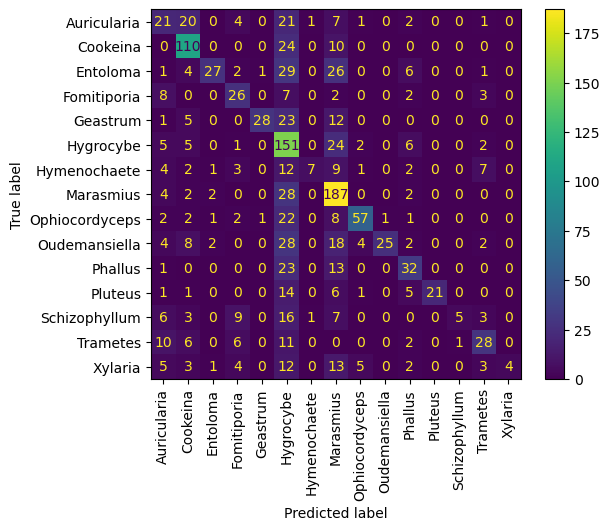
\includegraphics[width=0.6\textwidth]{figures/baseline_matrix.png}
    \end{center}
    \caption{Random forest confusion matrix}
\end{figure}

\subsection{Primary Model}
\begin{figure}[h]
    \begin{center}
    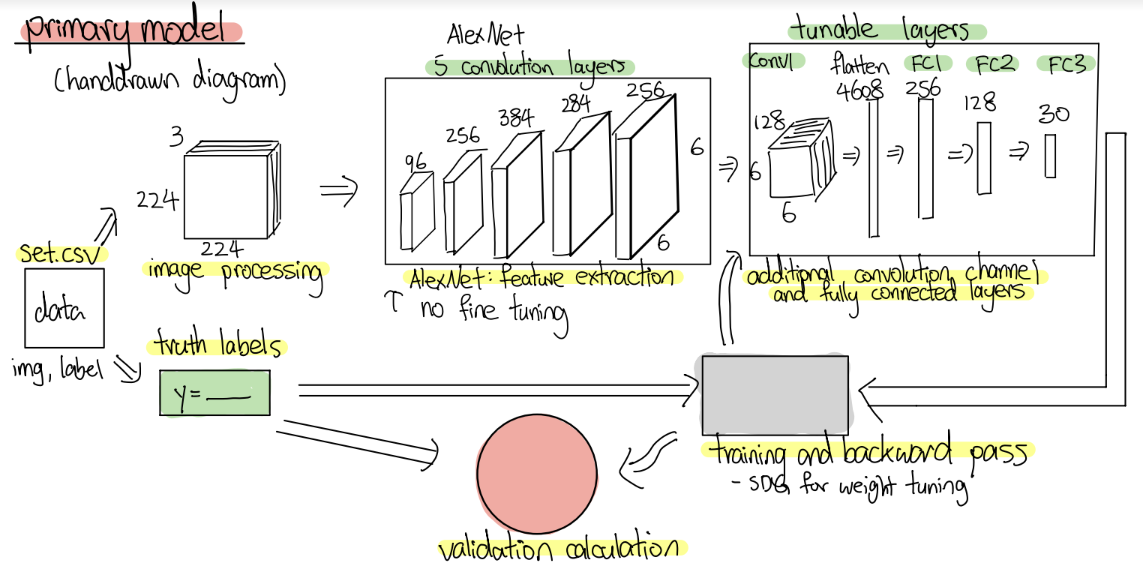
\includegraphics[width=0.9\textwidth]{figures/primaryModelDiagram.png}
    \end{center}
    \caption{Model Structure and Tensor Sizes}
\end{figure}


Our CNN model consists of two main sections: a non-tunable transfer learning part and a tunable convolution and fully connected layers section.

\subsubsection{Non-Tunable Section}
  
The team uses AlexNet for its high-level feature extraction. AlexNet processes a $3 \times 244 \times 244$ input image and the feature extraction outputs a $256 \times 6 \times 6$ tensor \citep{Bangar.AlexNetArchitectureExplained.2022}. There are five convolutional layers and three pooling layers \citep{Bangar.AlexNetArchitectureExplained.2022}, the order of the layers is shown on the hand-drawn diagram above. Since the model needs to differentiate between mushrooms with very similar appearances, AlexNet excels in extracting the fine features that set them apart.
  
\subsubsection{Tunable Section}
  
To make the model specific to the team’s project, the team uses one additional convolutional layer, outputting a $128 \times 6 \times 6$ tensor. After the additional convolutional layer, the output gets flattened and passed through three fully connected layers with ReLU activation functions in between. The fully connected layers turned the size from 4608 to 256, then to 128, and lastly to 30, matching the number of output classes the team decided for the model.
  

In total, there are $5+3$ layers in the non-tunable section and $1+3$ layers in the tunable section, making our class structure 12 layers in total.
  
\begin{figure}[h]
    \begin{center}
    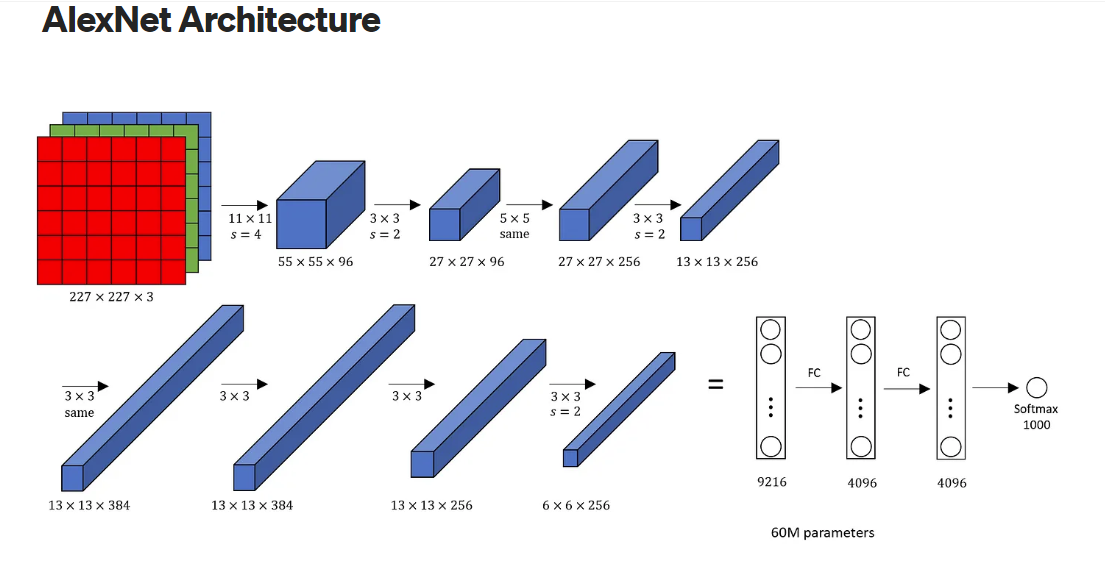
\includegraphics[width=0.6\textwidth]{figures/AlexNetStructure.png}
    \end{center}
    \caption{Class Structure: AlexNet \citep{Bangar.AlexNetArchitectureExplained.2022}}
\end{figure}

\subsubsection{Calculation of Parameters}

\subsubsubsection{Number of parameters for the AlexNet structure:}
\begin{align*}
\text{Conv1} & = 3 \times 11 \times 11 \times (96 + 1) = 35,271 \\
\text{Conv2} & = 96 \times 5 \times 5 \times (256 + 1) = 616,800 \\
\text{Conv3} & = 256 \times 3 \times 3 \times (384 + 1) = 886,080 \\
\text{Conv4} & = 384 \times 3 \times 3 \times (384 + 1) = 1,310,720 \\
\text{Conv5} & = 384 \times 3 \times 3 \times (256 + 1) = 887,232 \\
\end{align*}

\subsubsection{Number of parameters for the tunable section:}
\begin{align*}
\text{Conv1} & = 256 \times 3 \times 3 \times (128 + 1) = 297,216 \\
\text{Fc1} & = 4608 \times (256 + 1) = 1,183,296 \\
\text{Fc2} & = 256 \times (128 + 1) = 33,024 \\
\text{Fc3} & = 128 \times (30 + 1) = 3,968 \\
\end{align*}

The total number of parameters is 5,273,927, the number of trainable parameters is only 1,517,504. This ensures the training time for our models is feasible, allowing the team to focus on more epochs and more variations using data augmentations in the future.

At the start, the team pushed all images into the feature extraction part of AlexNet, converting data into tensors. We randomly split the data into a 75\%, 15\%, and 10\% ratio for training, validation, and testing.

For our current best result, we used a batch size of 36, learning rate of 0.007, and 15 epochs. We chose Cross Entropy Loss for the loss function as we want the model to classify the image into one of the 30 classes. For the optimizer, the group decided on Stochastic Gradient Descent (SGD).

\begin{figure}[h]
    \begin{center}
    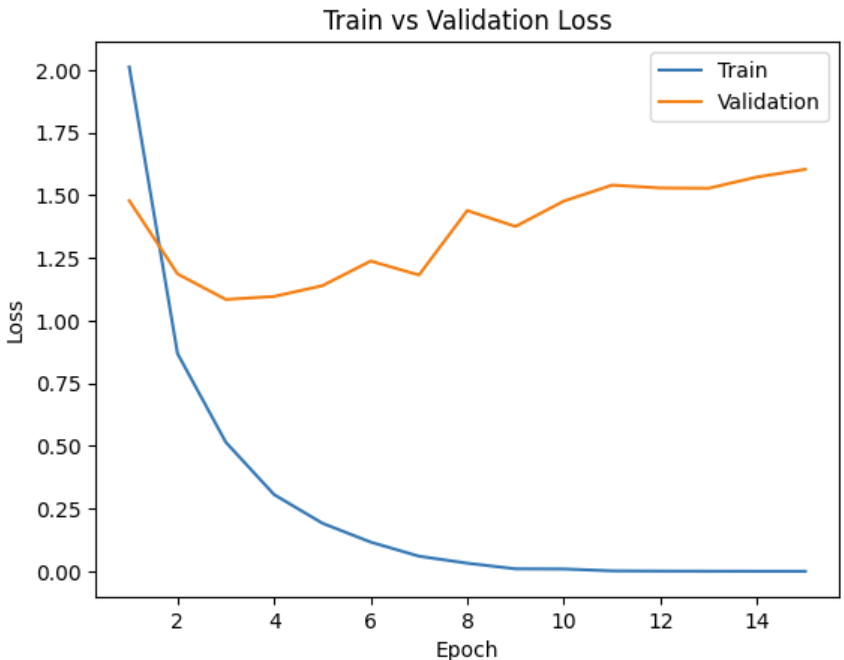
\includegraphics[width=0.6\textwidth]{figures/validationLossGraph.png}
    \end{center}
    \caption{Validation Loss}
\end{figure}

The team's training graph with the specified hyper-parameters is shown above. It indicates that the model is overfitted quickly, to tackle this issue, the team aims to implement regularization and drop off in the future.

\textbf{Testing Accuracy:}
\begin{itemize}
    \item Epoch 4: Test Classification Accuracy: 64.01\%
    \item Epoch 8: Test Classification Accuracy: 65.12\%
\end{itemize}

From the above graph, the team chose epochs 4 and epoch 8 and did accuracy testing, using the testing data. The testing accuracy is at a good starting point considering the model must classify an image into one of thirty classes. The accuracy can be improved using various techniques:
\begin{itemize}
    \item The current data used in the training is not augmented. The data augmentation functions are completed, but not used currently to save runtime for the training loop. The team will add the augmented data as part of training in the future.
    \item Further hyperparameters fine tuning.
    \item Implementing regularization and drop off to reduce the quick overfitting seen in the validation graph.
\end{itemize}


\label{last_page}

\bibliography{progress_ref}
\bibliographystyle{iclr2022_conference}

\end{document}
